\documentclass{beamer}

\usepackage{cite,doi}
\usepackage{amsmath,amssymb,amsfonts}
\usepackage{algorithm,algpseudocode}
\usepackage{stackengine,graphicx}
\usepackage{textcomp}
\usepackage{xcolor}
\usepackage{cleveref}
\usepackage{tikz}
\usetikzlibrary{3d}
\usetikzlibrary{patterns}
\usetikzlibrary{calc}
\usetikzlibrary{arrows}
\usetikzlibrary{matrix}
\usetikzlibrary{positioning}
\usetikzlibrary{decorations.pathreplacing}
\usepackage{mathtools}
\usepackage{subcaption}
\usepackage{import}
\usepackage{bm}
\usepackage[mathscr]{eucal}
\usepackage{amsbsy}
\usepackage[section]{placeins}
\usepackage{adjustbox}
\stackMath

\usepackage{../ourmacros}

\newcommand{\T}[1]{\boldsymbol{\mathscr{#1}}}

\newcommand{\GB}[1]{\textcolor{red}{\textbf{GB}: #1}}
\newcommand{\hyper}{DC-HYDICE}
\newcommand{\image}{SIIM-ISIC}

\definecolor{wfugold}{rgb}{0.6196078,0.494117647,0.21960784}
\newcommand{\red}[1]{\textcolor{red}{#1}}
\newcommand{\blue}[1]{\textcolor{blue}{#1}}
\newcommand{\multiplycolor}{red}
\newcommand{\zero}{}
\newcommand{\cred}[1]{\textcolor{red}{#1}}
\newcommand{\cblue}[1]{\textcolor{blue}{#1}}
\newcommand{\cgold}[1]{\textcolor{wfugold}{#1}}
\newcommand{\email}[1]{\href{mailto:#1}{\texttt{#1}}}


\newlength\matfield
\newlength\tmplength
\def\matscale{1.}
\newcommand{\dimbox}[3]{%
  \setlength\matfield{\matscale\baselineskip}%
  \setbox0=\hbox{\vphantom{X}\smash{#3}}%
  \setlength{\tmplength}{#1\matfield-\ht0-\dp0}%
  \fboxrule=1pt\fboxsep=-\fboxrule\relax%
  \fbox{\makebox[#2\matfield]{\addstackgap[.5\tmplength]{\box0}}}%
}
\newcommand{\raiserows}[2]{%
   \setlength\matfield{\matscale\baselineskip}%
   \raisebox{#1\matfield}{#2}%
}
\newcommand{\matbox}[5]{
  \stackunder{\dimbox{#1}{#2}{$#5$}}{\scriptstyle(#3\times #4)}%
}

\title{Parallel Hierarchical Clustering using \\ Rank-Two Nonnegative Matrix Factorization}

\author{
    Lawton Manning\inst{1}
    \and Grey Ballard\inst{1}\\
    \and Ramakrishnan Kannan\inst{2}
    \and Haesun Park\inst{3}
}

\institute{
    \inst{1}%
    Wake Forest University
    \and
    \inst{2}%
    Oak Ridge National Laboratory
    \and
    \inst{3}%
    Georgia Institute of Technology
}

\date{
    27th IEEE International Conference on High Performance Computing, Data, \& Analytics (HiPC 2020)
}

\usetheme{Warsaw}
\usecolortheme[named=wfugold]{structure}
%Madrid
%\usecolortheme{dolphin}
%\useinnertheme{rounded}
%\usefonttheme{serif}
\setbeamertemplate{navigation symbols}{} % gets rid of navigation bars
\setbeamertemplate{footline}
{
  \hbox{%
  \begin{beamercolorbox}[wd=.33\paperwidth,ht=2.25ex,dp=1ex,left]{author in head/foot}%
    \usebeamerfont{author in head/foot}
    Manning, Ballard, Kannan, Park
  \end{beamercolorbox}%
  \begin{beamercolorbox}[wd=.34\paperwidth,ht=2.25ex,dp=1ex,center]{title in head/foot}%
    \usebeamerfont{title in head/foot}
    HiPC 2020
  \end{beamercolorbox}%
  \begin{beamercolorbox}[wd=.33\paperwidth,ht=2.25ex,dp=1ex,right]{date in head/foot}%
    \usebeamerfont{date in head/foot}
    \insertframenumber{} \hspace*{2ex} 
  \end{beamercolorbox}}%
}


\begin{document}

\frame{\titlepage}

\begin{frame}{Summary}

    \begin{itemize}
        \item Nonnegative data can be hierarchically clustered using recursive bipartitioning based on Rank-2 Nonnegative Matrix Factorization (R2-NMF)
        \vfill
        \item Scalable parallelization requires efficient iterative algorithm for R2-NMF as well as data distribution conducive to data-dependent hierarchy structure
        \vfill
        \item Our approach scales well to 1000s of cores and is able to cluster 800GB image dataset
    \end{itemize}
    
\end{frame}

\begin{frame}{Nonnegative Matrix Factorization (NMF) for Clustering}
    \begin{adjustbox}{max totalsize={.4\textwidth}{.5\textheight},center}
    \import{..}{fig/nmf}
    \end{adjustbox}
    \begin{itemize}
        \item approximate $\M{A}$ (features $\times$ samples) into $\M{W}$ (features $\times$ clusters) and $\M{H}$ (samples $\times$ clusters)
        \vfill
        \item nonnegativity gives interpretability of $\M{W}$ and $\M{H}$ as clusters and cluster membership, respectively
        \vfill
        \item applications in text document topic modeling and hyperspectral image segmentation, for example
    \end{itemize}
\end{frame}

\begin{frame}{Hierarchical NMF}

\begin{itemize}
	\item repeatedly use NMF with $k = 2$ to bipartition nodes in order to create a hierarchical tree of clusters
	\item application: hyperspectral imaging
\end{itemize}

\begin{columns}
\begin{column}{.4\textwidth}
\GB{put bigger picture of DC mall (node 0) here, add pointers to leaves of tree for particular material (like grass or water)}
\end{column}
\begin{column}{.6\textwidth}
	\begin{adjustbox}{width=\textwidth}
    		\import{..}{fig/dc}
   	\end{adjustbox}
\end{column}
\end{columns}

\end{frame}

\begin{frame}{Solving NMF}
    \begin{itemize}
        \item NMF constrained optimization problem: $$\min_{\M{W},\M{H}\geq \M{0}} \|\M{A} - \M{W}\M{H}^\Tra\|_2$$
        
        \vfill
        
        \item Alternating Nonnegative Least Squares (ANLS)
        \begin{itemize}
            \item fix $\M{H}$ and solve the NLS for $\M{W}$ exactly
            \item alternate and repeat until convergence
        \end{itemize}
        
        \vfill

        \item General rank case
        \begin{itemize}
            \item can solve each row exactly using iterative active-set method
            \item determine which values are positive and which are zero
        \end{itemize}
        
        \vfill
        
         \item Rank-2 case
        \begin{itemize}
            \item 4 possibilities: both positive, one or other is zero, both zeroes 
            \item quickly solve each and choose the optimal solution
        \end{itemize}
    \end{itemize}
\end{frame}

\begin{frame}{Parallel R2-NMF}
    \begin{itemize}
        \item Use row distribution of $\M{A}$ and row distributions for $\M{W}$ and $\M{H}$ 
        \item Computational bottlenecks are matrix multiplications
        \begin{itemize}
            \item compute $\M{W}^\Tra\M{A}$ using reduce-scatter for $\M{H}$
            \item compute $\M{A}\M{H}$ using all-gather for $\M{W}$
            \item compute $\M{W}^\Tra\M{W}$ and $\M{H}^\Tra\M{H}$ using all-reduce
        \end{itemize}
    \end{itemize}
        \import{..}{fig/r2nmf}
\end{frame}

\begin{frame}{Bipartitioning with R2-NMF}
    \begin{itemize}
        \item Use columns of $\M{H}^\Tra$ to bipartition the columns of $\M{A}$
        \item Assign the cluster columns into two submatrices
        \item Assign columns of $\M{W}$ as feature signatures of clusters
    \end{itemize}
    \begin{adjustbox}{max totalsize={.7\textwidth}{.6\textheight},center}
        \import{..}{fig/split}
    \end{adjustbox}
\end{frame}

\begin{frame}{Hierarchical Clusterings using R2-NMF (HierNMF2)}
    \begin{itemize}
        \item Split root node into two children with R2-NMF
        \item Choose next node to split based on scoring metric
        \begin{itemize}
        		\item computing score requires pre-computing R2-NMF
	\end{itemize}
        \item Repeat until maximum number of frontier nodes is reached
    \end{itemize}
    \begin{adjustbox}{max totalsize={.7\textwidth}{.6\textheight},center}
        \import{..}{fig/tree}
    \end{adjustbox}
\end{frame}

\begin{frame}{Experimental Data Sets}
    \begin{itemize}
        \item DC-HYDICE
        \begin{itemize}
            \item Hyperspectral Digital Imagery Collection Experiment (HYDICE) of the National Mall in Washington, DC
        \end{itemize}
        \vfill
        \item SIIM-ISIC
        \begin{itemize}
            \item Society for Imaging Informatics in Medicine - International Skin Imaging Colloboration image classification of melanoma images
        \end{itemize}
        \vfill
        \item Synthetic Image classification
        \begin{itemize}
            \item smaller image classification dataset which has the same aspect ratio as SIIM-ISIC but fits in one node's memory
        \end{itemize}
    \end{itemize}
    \vfill
    \begin{center}
    \scriptsize
    	All experiments performed on Summit at Oak Ridge Leadership Computing Facility
    \end{center}
\end{frame}

\begin{frame}{R2NMF Strong Scaling}
    \centering
    \begin{columns}
        \begin{column}{0.5\textwidth}
            \begin{figure}
            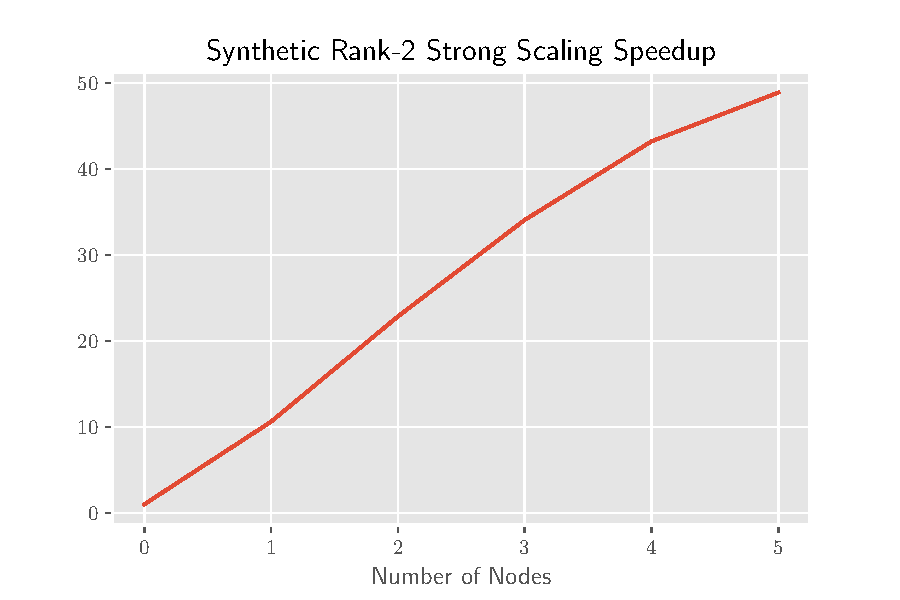
\includegraphics[width=\textwidth]{../plots/synthetic_rank2_speedup.pdf}
            \caption{Synthetic  Data}
            \end{figure}
        \end{column}
        \begin{column}{0.5\textwidth}
            \begin{figure}
            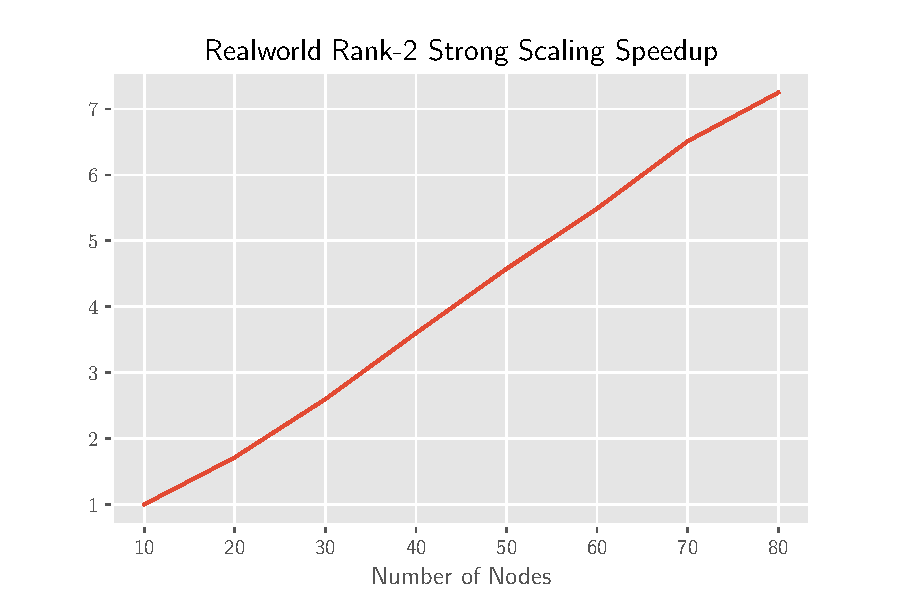
\includegraphics[width=\textwidth]{../plots/realworld_rank2_speedup.pdf}
            \caption{\image{} Data}
            \end{figure}
        \end{column}
    \end{columns}
\end{frame}

\begin{frame}{R2NMF Scaling Time Breakdowns}
    \centering
    \begin{columns}
        \begin{column}{0.5\textwidth}
            \begin{figure}
            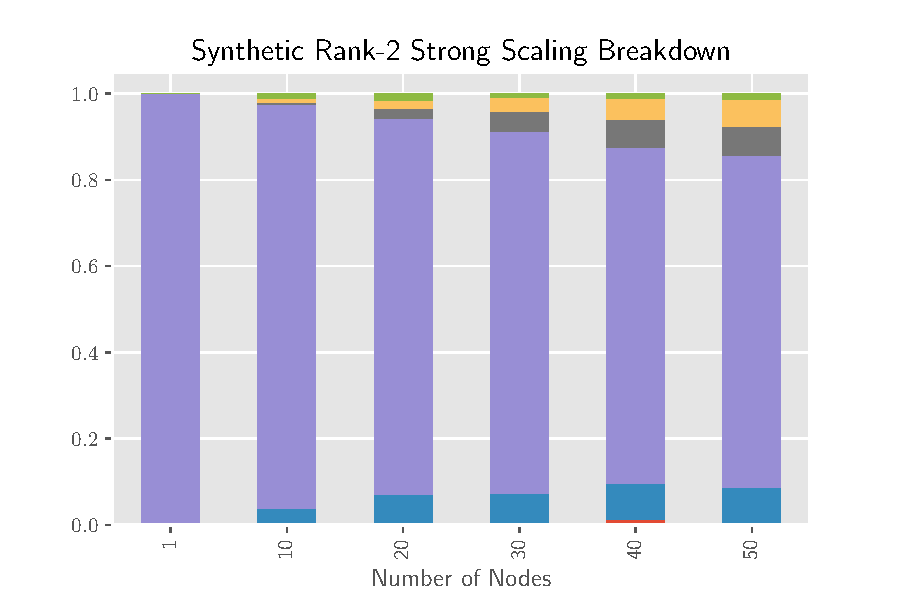
\includegraphics[width=\textwidth]{../plots/synthetic_rank2_strongscaling.pdf}
            \caption{Synthetic  Data}
            \end{figure}
        \end{column}
        \begin{column}{0.5\textwidth}
            \begin{figure}
            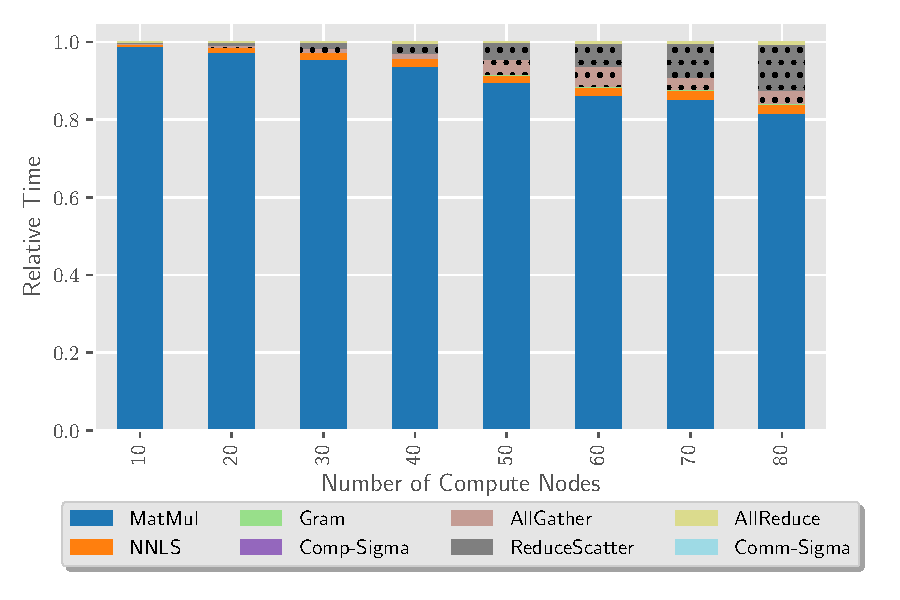
\includegraphics[width=\textwidth]{../plots/realworld_rank2_strongscaling.pdf}
            \caption{\image{} Data}
            \end{figure}
        \end{column}
    \end{columns}
\end{frame}

\begin{frame}{HierNMF Strong Scaling}
    \centering
    \begin{columns}
        \begin{column}{0.5\textwidth}
            \begin{figure}
            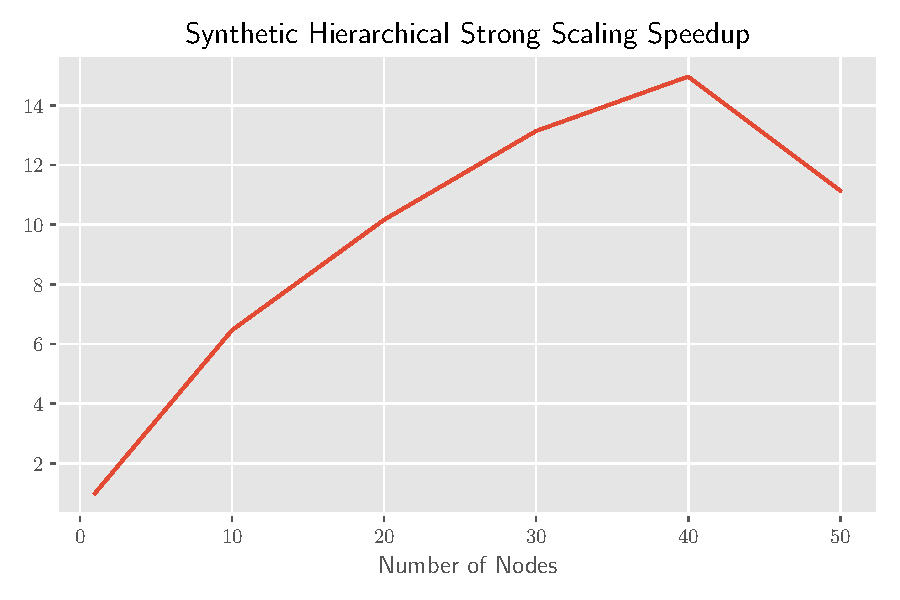
\includegraphics[width=\textwidth]{../plots/synthetic_hierarchical_speedup.pdf}
            \caption{Synthetic  Data}
            \end{figure}
        \end{column}
        \begin{column}{0.5\textwidth}
            \begin{figure}
            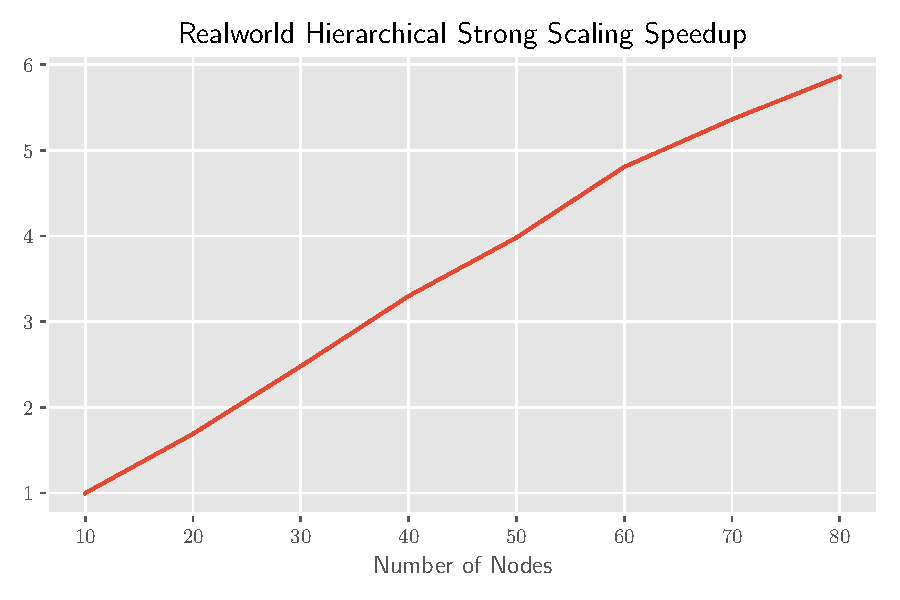
\includegraphics[width=\textwidth]{../plots/realworld_hierarchical_speedup.pdf}
            \caption{\image{} Data}
            \end{figure}
        \end{column}
    \end{columns}
\end{frame}

\begin{frame}{HierNMF Scaling Time Breakdowns}
    \centering
    \begin{columns}
        \begin{column}{0.5\textwidth}
            \begin{figure}
            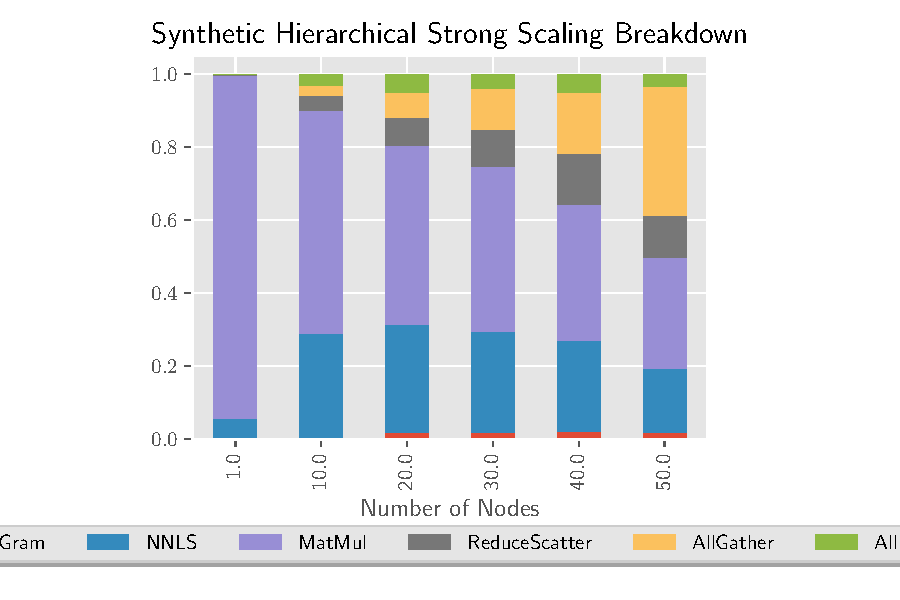
\includegraphics[width=\textwidth]{../plots/synthetic_hier_strongscaling.pdf}
            \caption{Synthetic  Data}
            \end{figure}
        \end{column}
        \begin{column}{0.5\textwidth}
            \begin{figure}
            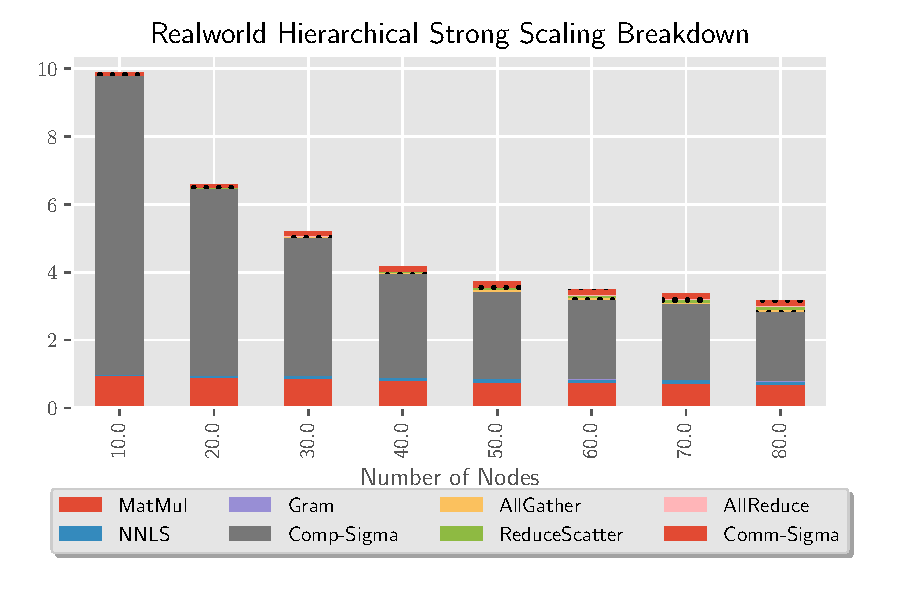
\includegraphics[width=\textwidth]{../plots/realworld_hier_strongscaling.pdf}
            \caption{\image{} Data}
            \end{figure}
        \end{column}
    \end{columns}
\end{frame}

\begin{frame}{Tree Level Times on Synthetic Data}
    \centering
    \begin{columns}
        \begin{column}{0.5\textwidth}
            \begin{figure}
            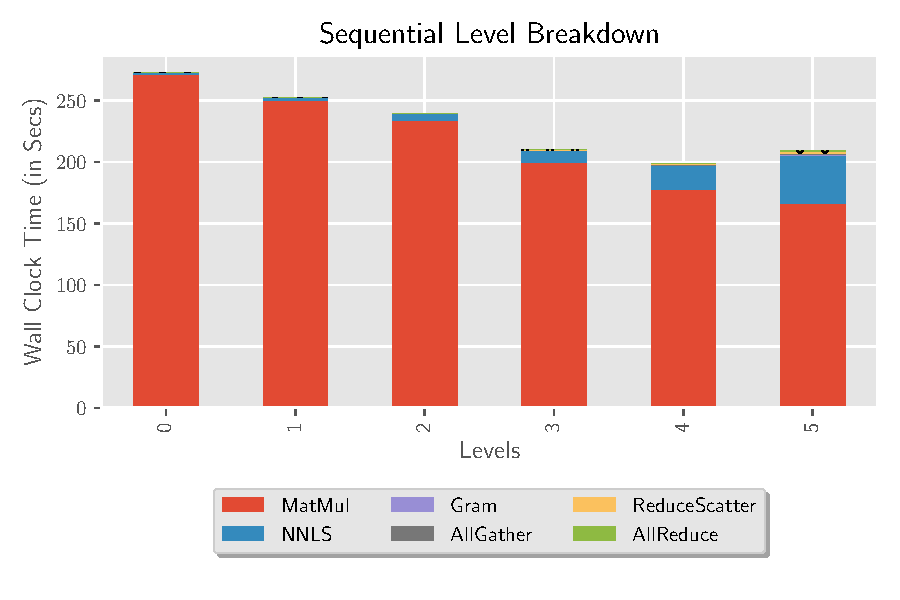
\includegraphics[width=\textwidth]{../plots/synthetic_sequential_level_breakdown.pdf}
            \caption{1 Compute Node}
            \end{figure}
        \end{column}
        \begin{column}{0.5\textwidth}
            \begin{figure}
            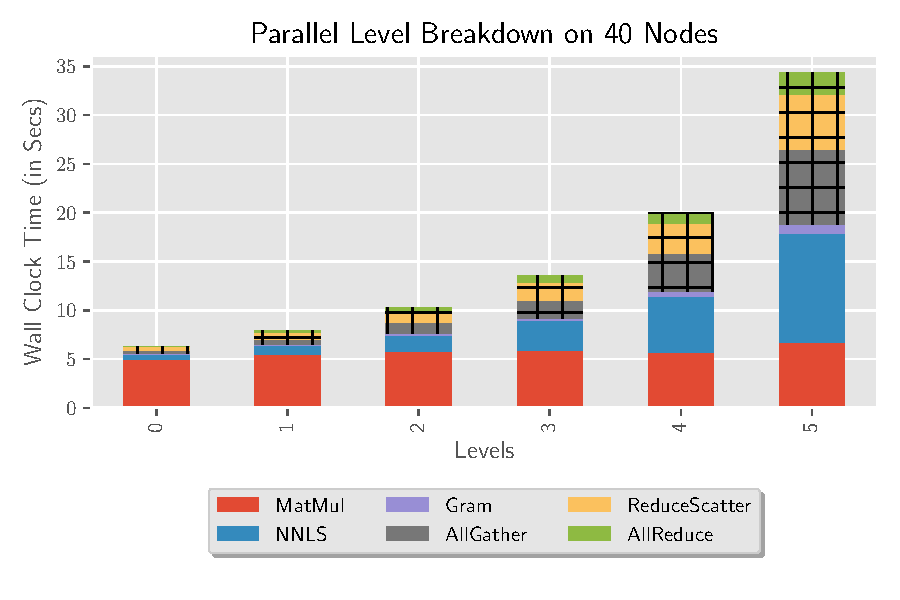
\includegraphics[width=\textwidth]{../plots/synthetic_parallel_level_breakdown.pdf}
            \caption{40 Compute Nodes}
            \end{figure}
        \end{column}
    \end{columns}
\end{frame}

\begin{frame}{Rank Scaling for Hierarchical and Flat NMF}
    \centering
    \begin{columns}
        \begin{column}{0.5\textwidth}
            \begin{figure}
            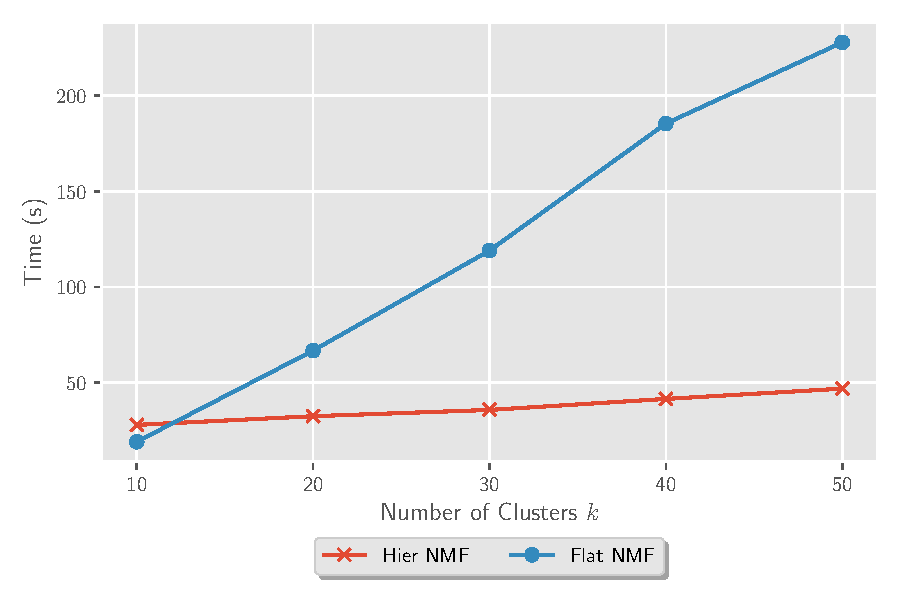
\includegraphics[width=\textwidth]{../plots/dc_rankscaling.pdf}
            \caption{\hyper{}  Data}
            \end{figure}
        \end{column}
        \begin{column}{0.5\textwidth}
            \begin{figure}
            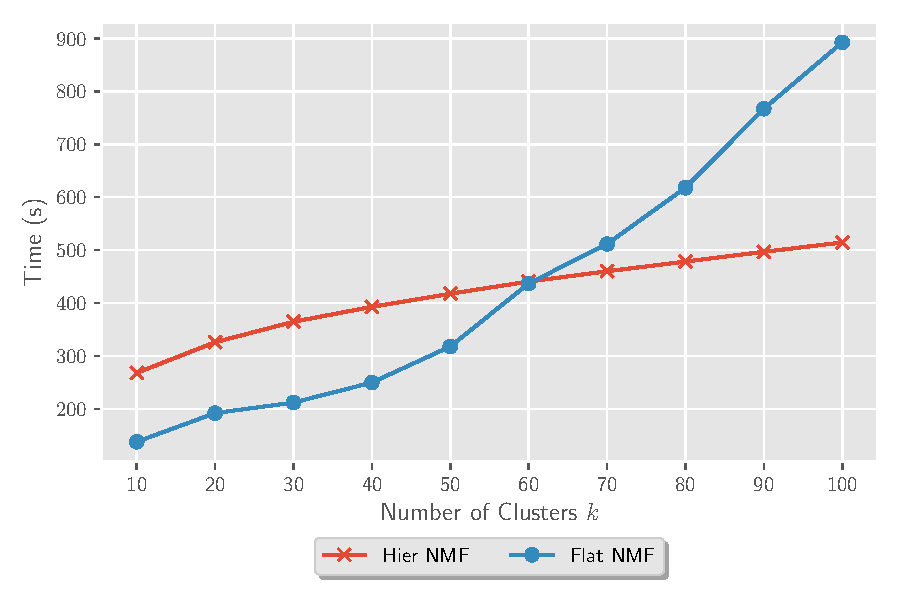
\includegraphics[width=\textwidth]{../plots/synthetic_rankscaling.pdf}
            \caption{Synthetic Data}
            \end{figure}
        \end{column}
    \end{columns}
\end{frame}



\begin{frame}
    \frametitle{Author Contact Information}
    
    For questions, please contact
    \begin{itemize}
        \item Lawton Manning: \email{mannlg15@wfu.edu}
        \item Grey Ballard: \email{ballard@wfu.edu}
        \item Ramakrishnan Kannan: \email{kannanr@ornl.gov}
        \item Haesun Park: \email{hpark@cc.gatech.edu}
    \end{itemize}
    
\end{frame}
    

\end{document}